This chapter describes the methodology used to generate counterfactual explanations using Variational Autoencoders (VAEs) and evaluate different feature masking strategies to enhance interpretability in autonomous driving systems. The methodology consists of multiple stages, including dataset collection, VAE training, classifier training, feature masking, counterfactual explanation generation.

A high-level workflow of the methodology is shown in Figure (let im edraw the methodology diagram and place an image). The dataset is collected from the CARLA simulator, preprocessed, and used to train a Variational Autoencoder (VAE) for latent space representation. A classifier is trained to distinguish between "STOP", "GO", "RIGHT, and "LEFT" decisions based on input images. Counterfactual explanations are generated by applying different feature masking techniques to alter the image or latent space representation. Finally, the counterfactuals are evaluated using both AI-based quantitative metrics and human evaluation studies.

\section{Experimental Setup}

All experiments in this thesis were conducted in a Linux environment to ensure compatibility with the CARLA simulator and associated tools. The setup was built using \textbf{CARLA version 0.9.15}, an open-source urban driving simulator widely adopted for autonomous driving research. This version provides a flexible and high-fidelity simulation environment, making it suitable for collecting diverse, labeled driving data under various rural and urban conditions.

To maintain compatibility with CARLA’s Python API, \textbf{Python version 3.7} was used for dataset collection. This version is recommended by CARLA’s developers to avoid API and dependency conflicts. The dataset was collected using two CARLA maps \textbf{Town03} and \textbf{Town07} \cite{CARLA2024}, provide varied driving topologies as shown in Figure~\ref{fig:carla_maps}. These maps were chosen due to their varied road layouts and environmental features, which provide rich scenarios for evaluating counterfactual explanations. Example simulation scenes demonstrating diverse driving and weather conditions are presented in Figure~\ref{fig:carla_scenes}. Users replicating this setup should download the CARLA server (v0.9.15) along with the additional maps from the \textit{official CARLA repository}. Once downloaded, the maps must be copied into the main CARLA directory to ensure proper integration.

\begin{figure}[htbp]
    \centering
    \begin{subfigure}{0.48\textwidth}
        \centering
        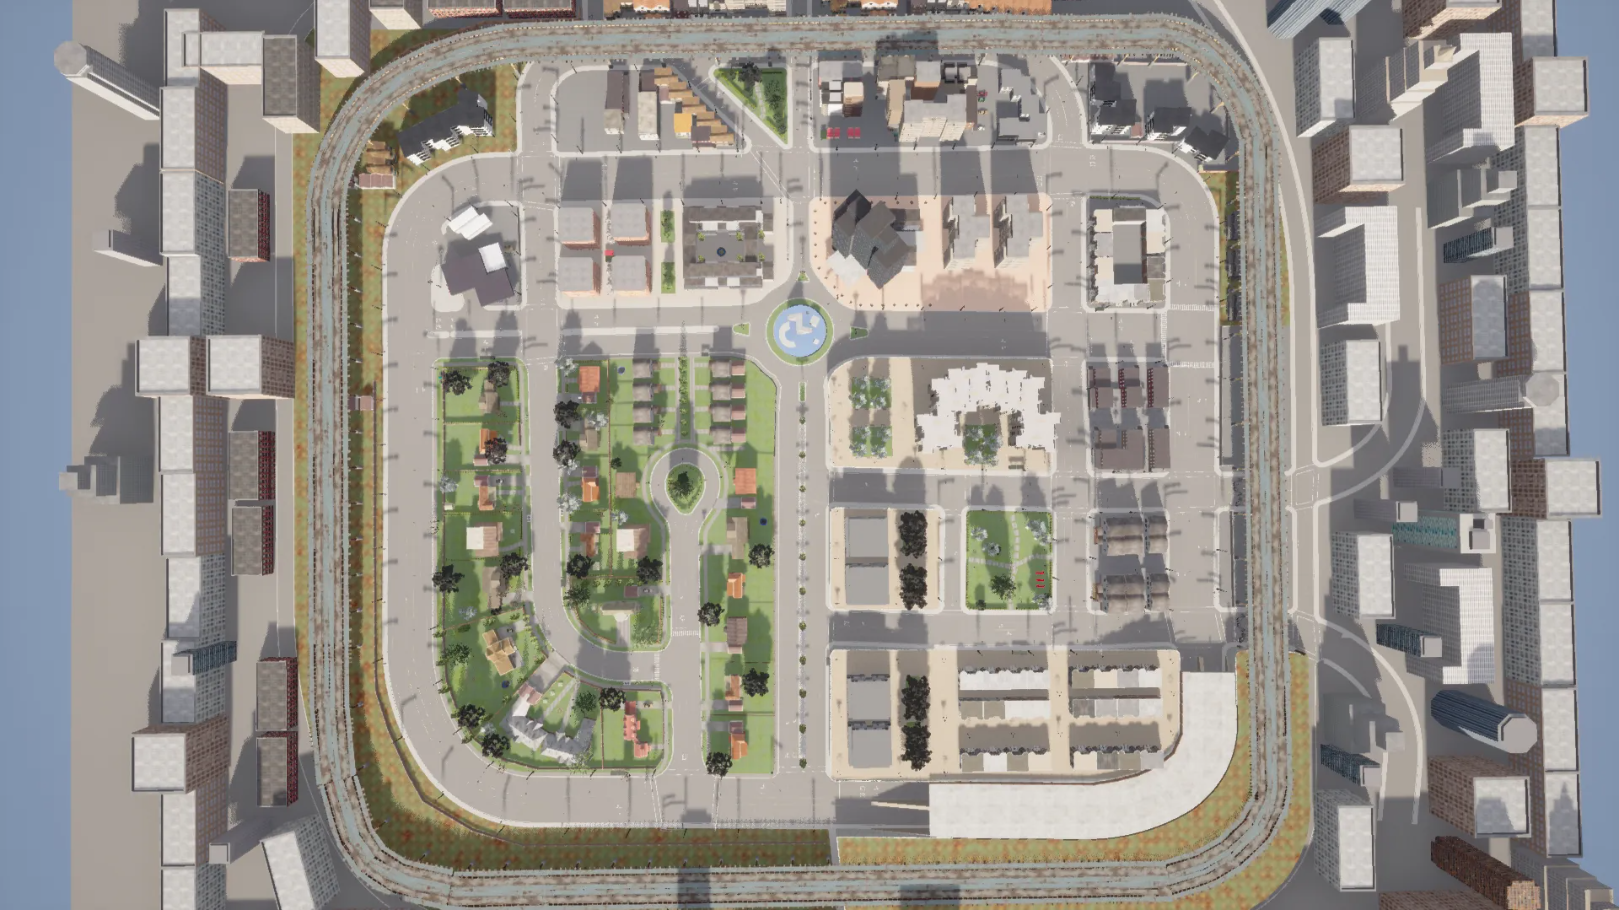
\includegraphics[width=\linewidth]{img/carla/town03.png}
        \caption{CARLA Town03 layout}
    \end{subfigure}
    \hfill
    \begin{subfigure}{0.48\textwidth}
        \centering
        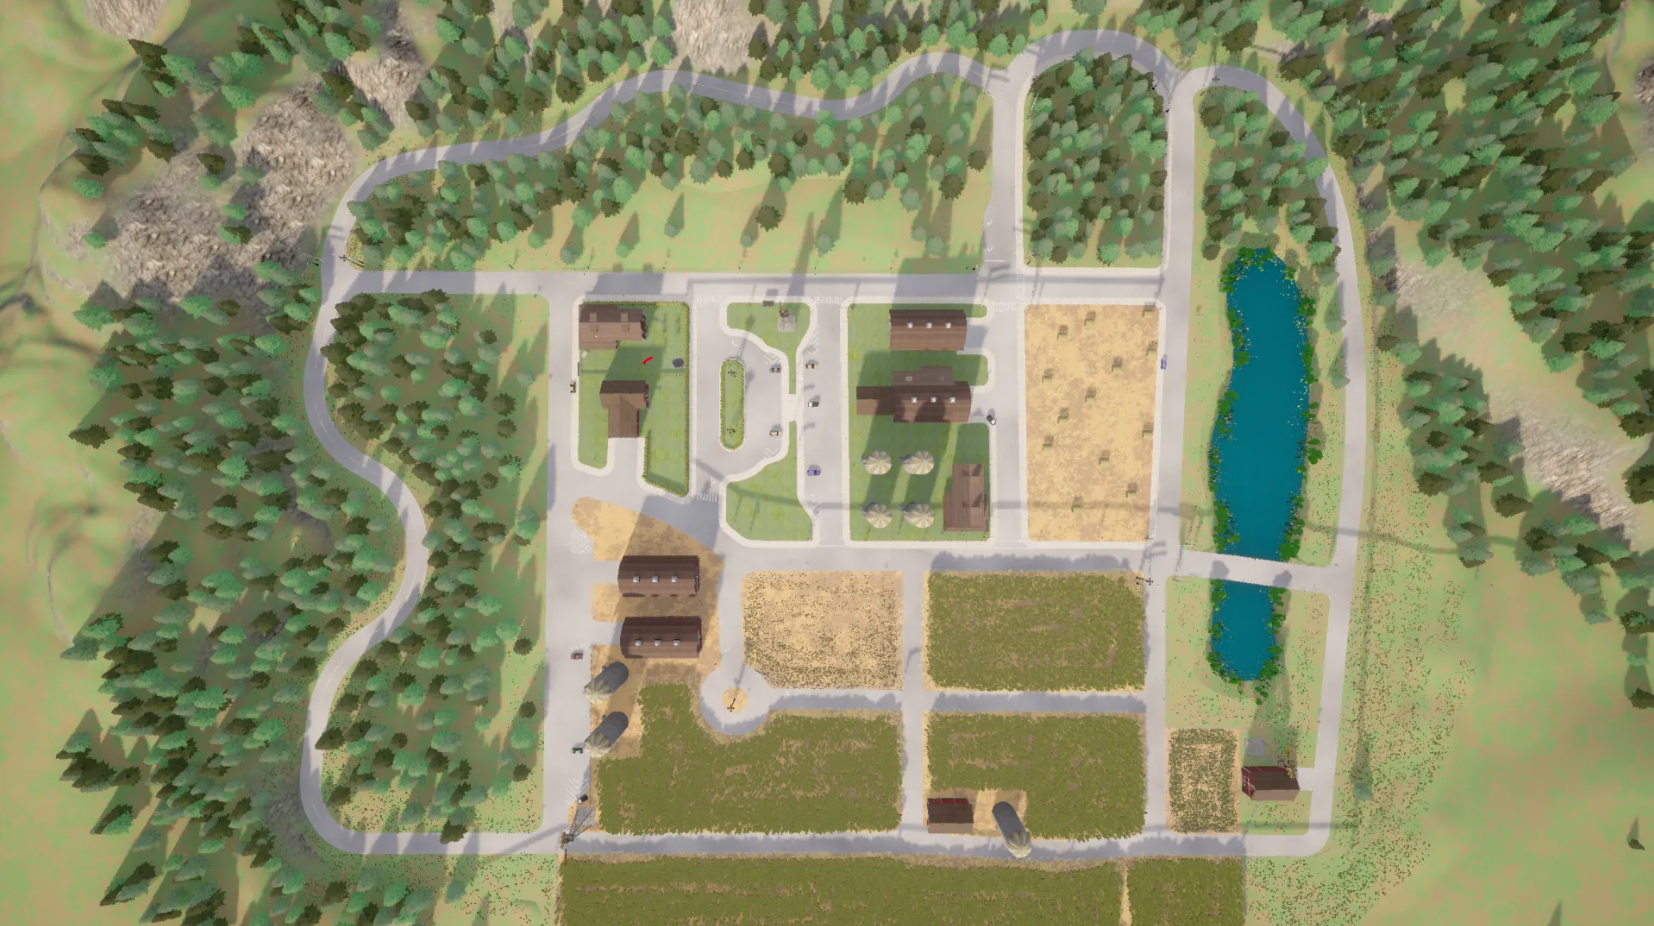
\includegraphics[width=\linewidth]{img/carla/town_7.png}
        \caption{CARLA Town07 layout}
    \end{subfigure}
    \caption{Top-down map layouts of the selected CARLA towns used for dataset collection~\cite{CARLA2024}}.
    \label{fig:carla_maps}
\end{figure}

\begin{figure}
    \centering
    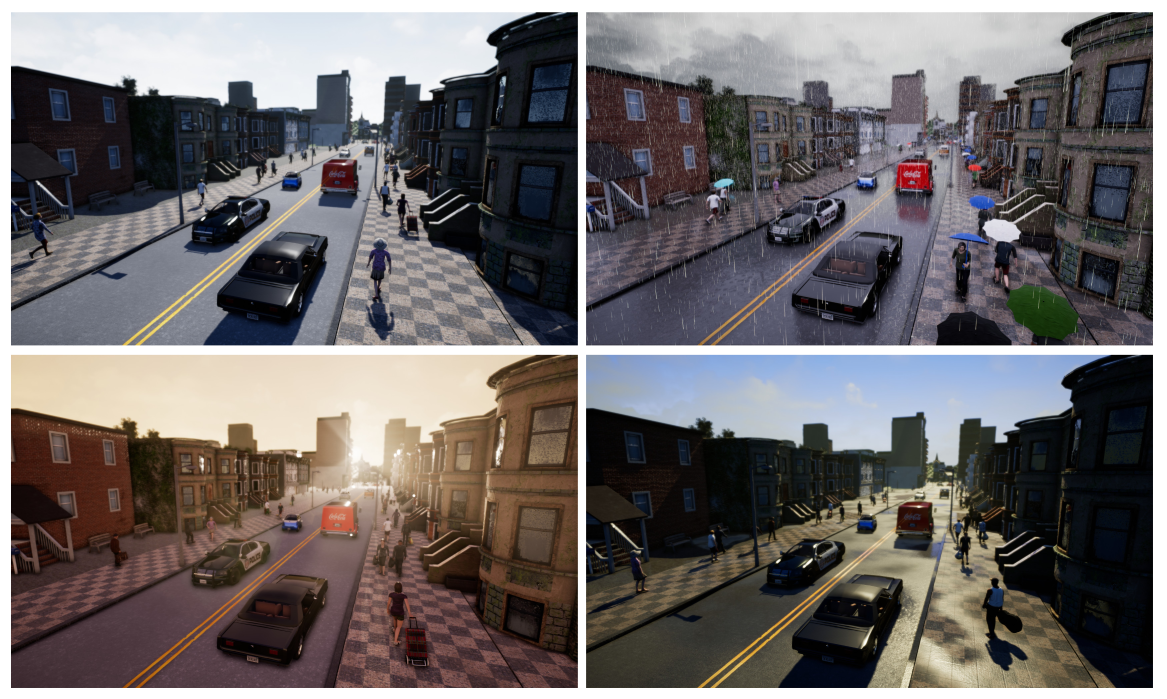
\includegraphics[width=0.7\linewidth]{img/carla/CARLA_Environment.png}
    \caption{3D Sample scenes from CARLA showcasing diverse conditions during dataset collection. The images illustrate a variety of urban and rural settings, with diverse lighting and weather conditions, including sunny, foggy, rainy, and snowy scenarios. Each scene highlights the flexibility of CARLA in simulating realistic driving environments for autonomous vehicle testing.}
    \label{fig:carla_scenes}
\end{figure}


Before executing any client-side scripts for dataset collection, it is essential to start the CARLA server using the following command in the CARLA root directory: ./CarlaUE4.sh


This launches the CARLA simulation in the Unreal Engine environment. For smooth operation, it is recommended to run the project on a system with at least \textbf{16 GB of RAM}, a dedicated GPU (e.g., \textbf{NVIDIA RTX series}), and \textbf{Ubuntu 18.04 or 20.04 LTS}. 

For the development and training of the Variational Autoencoder (VAE) and classifier models, we used \textbf{Python version 3.11 or higher}. This was necessary to avoid compatibility issues with newer versions of PyTorch, which are not well supported on older Python versions like 3.7. While dataset collection was handled using Python 3.7, the core machine learning model development required a more modern Python environment.  

To monitor and interpret various aspects of model training such as loss, accuracy, weight distributions, and layer activations we used \textbf{TensorBoard}. It provided valuable insights into training behavior and helped fine-tune model performance.

\section{Dataset Collection, Labeling, and Splitting Process}

To train and evaluate the proposed models effectively, a high-quality and well-structured dataset was essential. A systematic data preparation pipeline consisting of three key stages \textit{collection}, \textit{labeling}, and \textit{splitting}. The dataset was first collected using the CARLA simulator, which offers a controllable and realistic environment for simulating diverse driving scenarios. Following data collection, a precise rule-based labeling strategy was applied using vehicle control signals to assign meaningful class labels. Finally, the labeled dataset was partitioned into training and testing subsets to ensure class balance and prevent data leakage. This structured pipeline ensured consistency, and reproducibility  throughout the experimental workflow.

\subsection{Dataset Collection}

The dataset was collected using the CARLA simulator~\cite{CARLA2024docs}. An Audi A2 vehicle was deployed in autopilot mode to autonomously navigate the environment while capturing RGB images and corresponding control signals. A front mounted RGB camera was configured with a 125° field of view (FoV) and a resolution of $160 \times 80$ pixels. This resolution was selected to balance computational efficiency with sufficient visual detail for model learning.

A total of approximately 12,000 images were collected under varied driving scenarios. Each image was paired with the vehicle’s control parameters steering, throttle, and brake. The \textit{steering angle} ranged from $-1$ (full left) to $1$ (full right), while \textit{throttle} and \textit{brake} values ranged from $0$ to $1$, representing the intensity of acceleration and braking, respectively. This multi-modal data captured both visual context and driving behavior. The resulting dataset served as the foundation for both binary (STOP vs. GO) and multi-class (STOP, GO, LEFT, RIGHT) classification tasks.


\subsection{Dataset Labeling}

The collected data was labeled using a deterministic rule-based strategy derived from the vehicle’s control inputs. Two distinct labeling schemes were implemented to support binary and multi-class classification objectives.

For the \textbf{binary-class scheme}, each frame was labeled as either \texttt{STOP} or \texttt{GO}. A frame was labeled as \texttt{STOP} if the brake value exceeded a predefined threshold. Otherwise, it was labeled as \texttt{GO}. This distinction effectively captured the vehicle's motion state based on braking behavior.

For the \textbf{multi-class scheme}, labels were assigned based on prioritized control logic:
\begin{itemize}
    \item STOP, if the brake value exceeded a defined threshold.
    \item RIGHT, if the steering value was significantly positive and throttle was active.
    \item LEFT, if the steering value was significantly negative and throttle was active.
    \item GO, for all remaining cases where the vehicle moved straight without braking or significant steering.
\end{itemize}

This approach ensured mutually exclusive and semantically meaningful labels for each image. Threshold values for labeling were empirically determined based on the distribution of control signals across the dataset. The process was fully automated, ensuring reproducibility and eliminating manual labeling bias.

\subsection{Dataset Splitting}

Following labeling, the dataset was divided into separate training and testing subsets. The splitting was performed \textit{after} labeling to maintain label integrity and avoid any form of data leakage. Care was taken to ensure that the distribution of class labels remained balanced across both sets. This was critical for promoting fair learning and evaluation, particularly in the multi-class scenario.

The labeled dataset was partitioned using an 80/20 split ratio, where 80\% of the data was used for training and 20\% for testing. This ensured sufficient data for model learning while preserving a representative set for evaluation.

For the binary classification scheme, the training set contained 4,959 GO and 4,728 STOP samples, while the test set included 1,262 GO and 1,160 STOP samples, maintaining a near-balanced distribution across classes. Similarly, for the 4-class setting, all classes (GO, STOP, LEFT, RIGHT) were equally represented with 3,327 samples in training and 821 samples per class in testing. The distributions for both schemes are visualized side by side in Figure~\ref{fig:label_distribution_combined}.


\begin{figure}[htbp]
    \centering
    \begin{subfigure}{0.48\textwidth}
        \centering
        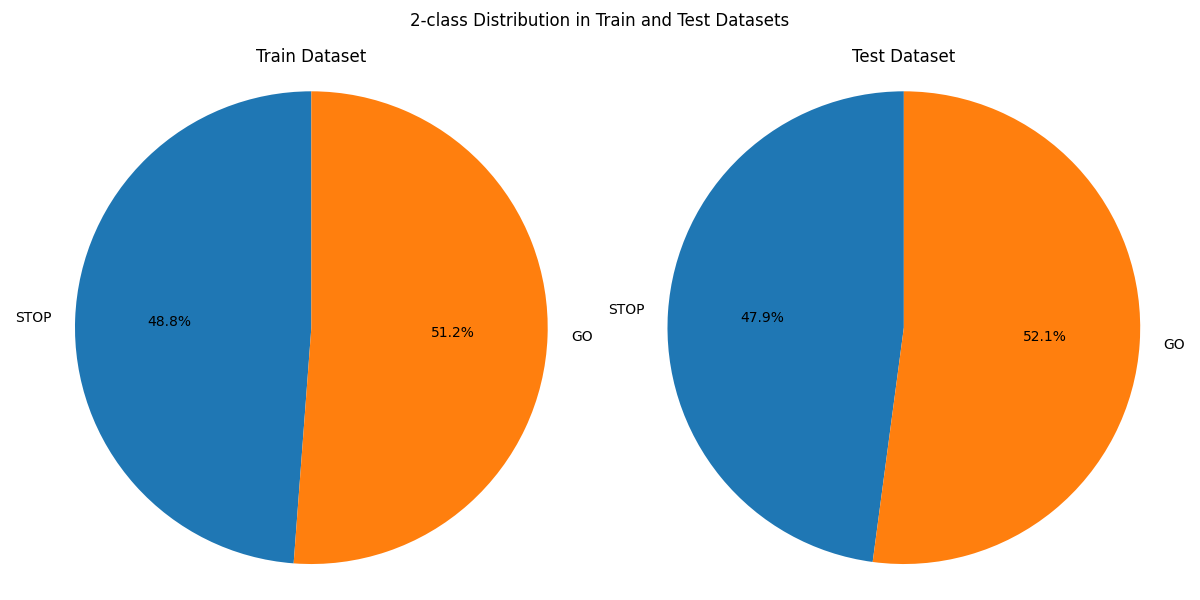
\includegraphics[width=\linewidth]{img/dataset/2class_distribution.png}
        \caption{Binary (GO/STOP) label distribution\vphantom{g}}
        \label{fig:binary_class_distribution}
    \end{subfigure}
    \hfill
    \begin{subfigure}{0.5\textwidth}
        \centering
        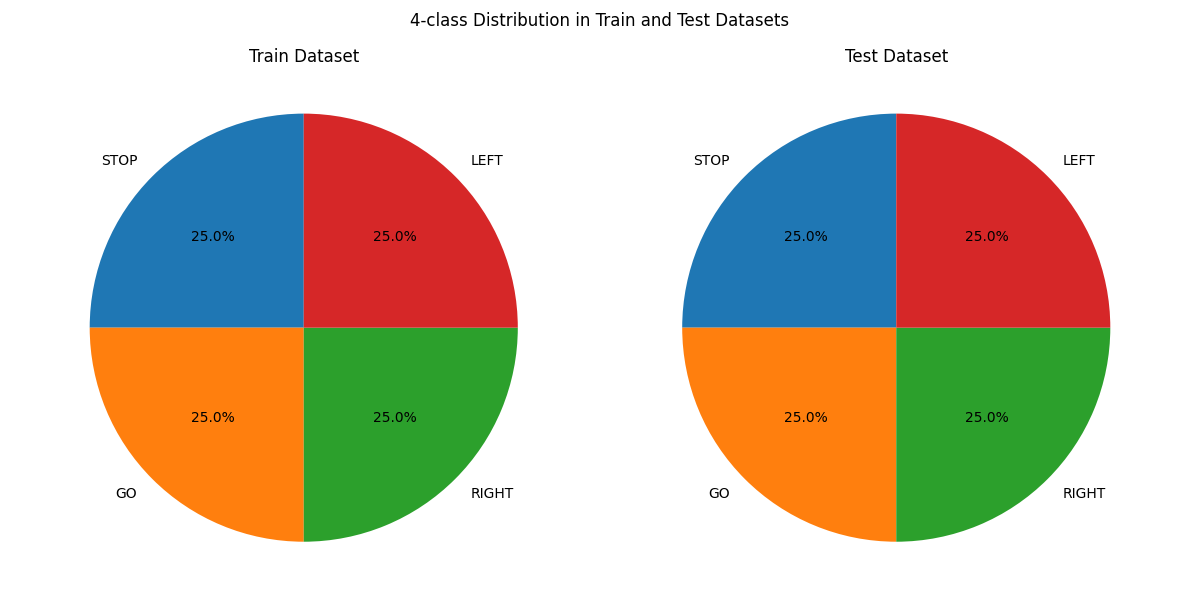
\includegraphics[width=\linewidth]{img/dataset/4class_distribution.png}
        \caption{4-class label distribution (GO, STOP, LEFT, RIGHT)}
        \label{fig:class_distribution_pie}
    \end{subfigure}
    \caption{Label distributions across training and testing datasets for binary and multi-class classification schemes.}
    \label{fig:label_distribution_combined}
\end{figure}





\section{Variational Autoencoder (VAE)} \label{sec:vae}

This section outlines the architectural design, training process, and evaluation protocol for the Variational Autoencoder (VAE) used in this work. The VAE serves as a generative backbone for producing realistic and plausible counterfactual explanations in the context of autonomous driving. Each component of the system is described in detail, along with the rationale for the chosen configurations and metrics.

To generate semantically coherent and visually realistic counterfactual explanations that remain on the data manifold, we adopt a Variational Autoencoder (VAE) as the generative backbone of our system. This approach draws conceptual motivation from the Contrastive Explanation Method (CEM)~\cite{DBLP:journals/corr/abs-1802-07623}, which leverages autoencoders to constrain generated samples within the support of the data distribution. While CEM was originally evaluated on low-dimensional datasets such as MNIST, our application domain involves high-resolution RGB images from complex driving scenarios. Consequently, the VAE architecture, training objective, and optimization strategy were carefully adapted and refined over multiple design iterations.

\subsection{VAE Architecture} \label{sec:vae_architecture}

The VAE consists of two primary components, a convolutional encoder that transforms the input image into a latent distribution, and a decoder that reconstructs the image from a sampled latent vector. The encoder and decoder are trained jointly using a variational loss function that enforces both reconstruction fidelity and latent space regularization.

\subsubsection{Encoder Architecture} \label{subsubsec:vae_encoder}

The encoder takes an input image of shape $3 \times 80 \times 160$ (RGB, height $\times$ width) and compresses it into a 128-dimensional latent space. The architecture is composed of four convolutional blocks followed by fully connected layers:

\begin{itemize}
    \item \textbf{Conv Layer 1:} 64 filters, kernel size $4 \times 4$, stride 2, no padding. Followed by LeakyReLU.
    \item \textbf{Conv Layer 2:} 128 filters, kernel size $3 \times 3$, stride 2, padding 1. Followed by BatchNorm and LeakyReLU.
    \item \textbf{Conv Layer 3:} 256 filters, kernel size $4 \times 4$, stride 2. Followed by LeakyReLU.
    \item \textbf{Conv Layer 4:} 512 filters, kernel size $3 \times 3$, stride 2. Followed by BatchNorm and LeakyReLU.
\end{itemize}

The final feature map output is flattened and passed through a fully connected layer with 1024 units (with LeakyReLU activation). From this, two separate linear layers output the mean vector $\mu \in \mathbb{R}^{128}$ and log-variance vector $\log\sigma^2 \in \mathbb{R}^{128}$, representing the parameters of the approximate posterior $q(z|x)$.

\subsubsection{Latent Sampling via Reparameterization Trick}
The latent vector $z$ is sampled using the reparameterization trick:
\begin{equation}
z = \mu + \sigma \cdot \epsilon, \quad \epsilon \sim \mathcal{N}(0, I)
\end{equation}
This allows gradient-based optimization through the stochastic sampling process, maintaining end-to-end differentiability. The encoder uses PyTorch’s native implementation of a normal distribution to sample $\epsilon$, and places the distribution tensors on the correct device (CPU or GPU).




\subsubsection{Decoder Architecture} \label{subsubsec:vae_decoder}

The decoder reverses the encoding process and reconstructs an image from the latent vector $z \in \mathbb{R}^{128}$. It consists of two fully connected layers followed by four transposed convolutional layers:

\begin{itemize}
    \item \textbf{Dense Layer 1:} Linear projection from 128 to 1024 units with LeakyReLU.
    \item \textbf{Dense Layer 2:} Linear projection from 1024 to $512 \times 4 \times 9 = 18432$ units, reshaped to $(512, 4, 9)$.
\end{itemize}

The reshaped feature map is then passed through:

\begin{itemize}
    \item \textbf{Deconv Layer 1:} 256 filters, kernel size $4 \times 4$, stride 2, padding 1, output padding (0,1). Followed by LeakyReLU.
    \item \textbf{Deconv Layer 2:} 128 filters, kernel size $4 \times 4$, stride 2, padding 1, output padding (1,1). Followed by LeakyReLU.
    \item \textbf{Deconv Layer 3:} 64 filters, kernel size $4 \times 4$, stride 2. Followed by LeakyReLU.
    \item \textbf{Deconv Layer 4:} 3 filters (RGB), kernel size $4 \times 4$, stride 2. Followed by Sigmoid activation.
\end{itemize}

The final output has shape $3 \times 80 \times 160$, matching the input dimensions. The Sigmoid activation ensures output values lie in the normalized $[0,1]$ range.

\subsubsection{Training Objective and Optimization Strategy} \label{subsubsec:vae_loss}

The training objective for the VAE is the variational loss function:
\[
\mathcal{L}_{\text{VAE}} = \mathcal{L}_{\text{recon}} + \lambda_{\text{KL}} \cdot \mathcal{L}_{\text{KL}}
\]

\paragraph{Reconstruction Loss:} \label{reconstruction_loss}
Two reconstruction losses were implemented and tested:
\begin{itemize}
    \item \textbf{Mean Squared Error (MSE):} Penalizes squared differences between the original and reconstructed pixel values. Suitable for pixel-level fidelity.
    \item \textbf{Log-Cosh Loss:} More robust to outliers, behaves like MSE for small errors and like MAE for large errors.
\end{itemize}
The use of Log-Cosh was empirically found to produce smoother reconstructions in early training phases. This is motivated by Chen et al.~\cite{chen2019log}. So, in this thesis comparison between the MSE loss and Log-cosh loss was implemented and compared between them. The results are discussed in the     .

\paragraph{KL Divergence:}
The KL divergence regularizes the latent distribution:
\[
\mathcal{L}_{\text{KL}} = -\frac{1}{2} \sum_{i=1}^{d} \left(1 + \log\sigma_i^2 - \mu_i^2 - \sigma_i^2\right)
\]
It encourages the approximate posterior $q(z|x)$ to stay close to the unit Gaussian prior $p(z) = \mathcal{N}(0, I)$.

\paragraph{KL Weight Annealing:}
To avoid early dominance of the KL term, we implement linear annealing:
\[
\lambda_{\text{KL}} = \min(\lambda_0 + \delta \cdot \text{epoch}, 1.0)
\]
where $\lambda_0 = 5 \times 10^{-5}$ and $\delta = 1 \times 10^{-4}$. This allows the model to prioritize reconstruction initially, and gradually introduce regularization.

\paragraph{Training Configuration:}
The VAE is implemented using PyTorch and trained in Python 3.11 on a Linux system an NVIDIA CUDA-enabled GPU (e.g., RTX 1080 Ti). Libraries include Torchvision, Matplotlib, NumPy, and PIL.

\begin{itemize}
    \item Optimizer: Adam
    \item Learning Rate: $1 \times 10^{-4}$; Weight Decay: $1 \times 10^{-5}$
    \item Batch Size: 128
    \item Epochs: 200
    \item Scheduler: \texttt{ReduceLROnPlateau} (patience = 10, factor = 0.5)
    \item Early Stopping: patience = 50
\end{itemize}

Each epoch logs training and validation losses (total, reconstruction, KL), pixel-level accuracy, and PSNR.

\subsection{Evaluating VAE Performance} \label{subsec:vae_evaluation}

Model performance is assessed using both quantitative and qualitative metrics:
\begin{itemize}
\item \textbf{Reconstruction Loss:} MSE or Log-Cosh.
\item \textbf{Pixel Accuracy:} Proportion of correctly reconstructed pixels after thresholding.
\item \textbf{PSNR:} Perceptual quality of reconstruction.
\item \textbf{Visual Inspection:} Periodic reconstruction samples are compared with ground truth.
\item \textbf{Latent Space Evaluation:} Interpolation and prior sampling validate structure and continuity.
\item \textbf{Training Curves:} Epoch-wise plots for all metrics enable trend analysis and convergence monitoring.
\end{itemize}

These evaluations confirm the VAE's capacity to learn expressive, structured representations, which are later used for counterfactual explanation in \autoref{Evaluation and Results}.



\section{Classifier Model for Prediction} \label{sec:classifier_mdel_for_prediction}
To assess the semantic structure of the learned latent space and evaluate downstream task performance, multiple classifiers were trained using the 128-dimensional latent representations generated by the VAE encoder. Each image corresponds to a driving situation (e.g., STOP, GO, RIGHT, LEFT), and the classifiers were trained to predict the appropriate driving action class from the latent vector.

Unlike conventional approaches where classifiers are trained directly on pixel-level image data, this work emphasizes feature-based classification, operating solely in the compressed and semantically meaningful latent space. This allows for efficient model training, improved interpretability, and compatibility with counterfactual explanation techniques explored later in the thesis.

Five classification models were implemented and evaluated:
\begin{itemize}
    \item \textbf{Neural Network (MLP):} A 3-layer fully connected network with LeakyReLU activations and dropout.
    \item \textbf{Logistic Regression:} A linear baseline model to establish separability in the latent space.
    \item \textbf{K-Nearest Neighbors (KNN):} A non-parametric, distance based model suitable for evaluating the local structure of the latent space.
    \item \textbf{Support Vector Machine (SVM):} A margin based classifier using a radial basis function kernel for better non-linear decision boundaries.
    \item \textbf{Random Forest:} An ensemble based decision tree model offering robustness and interpretability.
\end{itemize}

All classifiers were trained in both binary and multi-class settings. The binary setup involved classifying between \texttt{GO} and \texttt{STOP} scenarios, while the multi-class setup extended this to include \texttt{LEFT} and \texttt{RIGHT} actions, resulting in a four-class prediction task.

As detailed in Section~\ref{subsubsec:vae_encoder}, the encoder compresses each $3 \times 80 \times 160$ image into a 128-dimensional latent vector using a series of convolutional and fully connected layers. These latent vectors serve as inputs to all classifiers, forming the basis for prediction.

No pixel-level image information was used during classification. The models operate solely on the semantically rich latent space learned by the VAE. This aligns with the overall objective of this work: to build interpretable and compact representations that support both classification and counterfactual explanation generation.

\subsection{Classifier Architectures and Training Setup}

This section describes the architecture, training configurations, and optimization strategies used for each classifier. All models were trained and evaluated using the latent feature vectors extracted from the VAE encoder. The input to each classifier is a 128-dimensional feature vectors.

\subsubsection*{Neural Network Classifier (MLP)}

A deep feedforward neural network was implemented using PyTorch to classify the latent vectors extracted from the VAE. The architecture was designed with simplicity and effectiveness in mind, specifically tailored to the 128-dimensional latent representations. This classifier is composed of three fully connected (dense) layers, each followed by batch normalization and dropout regularization, with LeakyReLU activations throughout. The details are as follows:

\begin{itemize}
    \item \textbf{Input size:} 128 \\
    The input to the network is a 128-dimensional vector, corresponding to the latent features produced by the VAE encoder. This compact representation captures the essential semantic information from the original image.
    
    \item \textbf{Hidden layers:} 3 layers, each with 128 units \\
    Three fully connected hidden layers were chosen to provide the network with sufficient capacity to model non-linear relationships within the latent space. Maintaining a consistent layer size (128 units) aligns with the dimensionality of the latent vector, ensuring that each hidden layer can process the full feature set without dimensionality reduction, which helps preserve the rich information embedded in the latent space.
    
    \item \textbf{Activation:} LeakyReLU with slope 0.01 \\
    LeakyReLU is used as the activation function for its advantages over the traditional ReLU. Unlike ReLU, which zeroes out negative inputs, LeakyReLU allows a small, non-zero gradient (with a slope of 0.01) for negative values. This feature mitigates the "dying ReLU" problem, ensuring that neurons do not become inactive during training and thereby promoting better gradient flow across the network.
    
    \item \textbf{Regularization:} Dropout (p = 0.5) and Batch Normalization \\
    Dropout is applied with a probability of 0.5 after each hidden layer to prevent overfitting by randomly deactivating half of the neurons during training. This forces the network to learn more robust features that are not overly dependent on any single neuron. Batch Normalization is applied to stabilize and accelerate training by normalizing the inputs to each layer. It reduces internal covariate shift, which helps in achieving faster convergence and improved overall performance.
    
    \item \textbf{Output:} 2 or 4 logits depending on classification task \\
    The final output layer produces either 2 or 4 logits, corresponding to the binary or multi-class classification tasks, respectively. The logits represent the unnormalized scores for each class, and a softmax function is applied during loss computation (using CrossEntropy Loss) to obtain probability distributions over the classes.
\end{itemize}

This architecture was selected because it effectively balances model complexity and computational efficiency, making it well-suited for the compact and informative VAE latent space. By leveraging non-linear activations and regularization techniques, the network is capable of learning subtle distinctions between classes while mitigating overfitting, ultimately yielding strong classification performance.



\subsubsection*{Traditional Classifiers}

To compare the neural classifier's performance with classical machine learning models, the following classifiers were implemented using the scikit-learn library:

\begin{itemize}
    \item \textbf{Logistic Regression:} A linear classifier using the liblinear
    
    
    solver and L2 regularization.
    \item \textbf{K-Nearest Neighbors (KNN):} Set to $k=5$ using Euclidean distance.
    \item \textbf{Support Vector Machine (SVM):} RBF kernel with probability estimates enabled.
    \item \textbf{Random Forest:} Ensemble of 100 decision trees with a maximum depth determined automatically.
\end{itemize}

These models were trained on the same latent vectors as the neural network. The dataset was split into 80\% training and 20\% testing for evaluation. Metrics such as precision, recall, F1-score, confusion matrix, and ROC-AUC were computed for comprehensive analysis.

\subsubsection*{Binary vs Multi-Class Setup}

All classifiers were trained in two different settings:
\begin{itemize}
    \item \textbf{Binary Classification:} Predicting whether to \texttt{GO} or \texttt{STOP}, useful for early validation and simple decision-making.
    \item \textbf{Multi-Class Classification:} Predicting one of four classes: \texttt{STOP}, \texttt{GO}, \texttt{RIGHT}, or \texttt{LEFT}, enabling fine-grained driving behavior modeling.
\end{itemize}

Each setup used the same pipeline of latent feature extraction followed by classification. Evaluation was performed using the same data split and metrics across all models to enable a fair comparison.


\section{Feature Masking Techniques for Counterfactual Generation}
\label{sec:feature_masking_pipeline}

To generate counterfactual explanations (CEs), multiple feature masking strategies were employed, each with its own rationale, masking space (image or latent), and mechanism of perturbation. The objective in all these methods is consistent: identify minimal and plausible changes in the input that result in a different classification output, thus providing insight into the model decision boundary.

All methods follow a unified processing pipeline comprising the following steps:
\begin{enumerate}
    \item Encode the original image using a encoder of VAE to obtain a latent representation.
    \item Classify the latent vector using a trained classifier to obtain the original prediction.
    \item Apply a masking strategy (in image space or latent space).
    \item Reconstruct the masked or modified input using the decoder.
    \item Re-encode and classify the reconstructed image.
    \item Compare the new prediction with the original prediction. If different, a counterfactual explanation is identified.
\end{enumerate}

The masking strategies are categorized into two groups based on the space where the perturbation is applied.

\subsection*{Image Space Masking}
This includes Grid-Based Masking, LIME on Images, and Object Detection-Based Masking. These methods apply masking directly to the input image.
\begin{itemize}
    \item \textbf{Grid-Based Masking:} The image is divided into grids (e.g., 10$\times$5, 4$\times$2), and each cell is masked iteratively to observe prediction changes.
    \item \textbf{LIME on Images:} LIME is applied on pixel space to identify important regions, which are then masked.
    \item \textbf{Object Detection-Based Masking:} YOLOv5 is used to detect semantic objects (e.g., pedestrians, vehicles), which are then removed from the image by zeroing out pixels in the bounding box.
\end{itemize}

\subsection*{Latent Space Masking}
This includes LIME on Latent Features and LIME with nearest-unlike-neighbour (NUN). Here, perturbations are applied to the encoded latent vector.
\begin{itemize}
    \item \textbf{LIME on Latent Features:} LIME identifies influential latent dimensions. These are replaced using strategies such as median substitution or rule-based adjustments using dataset statistics.
    \item \textbf{LIME with NUN:} Combines LIME-based feature importance with the nearest-unlike-neighbour strategy, selecting feature replacements that are more robust and semantically meaningful.
\end{itemize}

For each method, similarity metrics (SSIM, PSNR, MSE, UQI, VIFP) are computed between the original and reconstructed images to assess visual fidelity. All results, including prediction changes, classifier confidences, masking parameters, and processing time, are logged into method-specific files for analysis. If the prediction changes after masking, the example is labeled as a successful counterfactual. This analysis directly supports answering the research question outlined in \cref{sec:research_question}, particularly \textbf{RQ3}.


In the subsequent subsections, each masking method is detailed along with its algorithm, implementation logic.
 

\subsection{Grid-Based Masking} \label{sec:grid_based_masking}

Grid-based masking is a spatial perturbation technique designed to generate counterfactual explanations (CEs) by selectively occluding small square regions of an input image. The underlying assumption is that certain spatial regions exert a disproportionate influence on the model’s classification decision. By masking these regions and observing changes in the model’s output, we can gain insights into which parts of the input image are causally relevant for the decision-making process.

This method follows the general feature masking pipeline outlined in Section~\ref{sec:feature_masking_pipeline}. First, the input image is encoded into a latent representation using a Variational Autoencoder (VAE). The latent features are passed to a classifier to generate the original prediction, and the image is also reconstructed via decoding for consistency. The masking operation is applied directly to the pixel space by zeroing out specific spatial regions (grid cells) before the image is re-encoded, reconstructed, and re-evaluated by the classifier.

To balance localization precision and computational efficiency, we experimented with multiple grid sizes and empirically selected two square grid configurations based on performance. 

\begin{itemize}
    \item \textbf{Fine grid:} $8 \times 16$ (each cell is $10 \times 10$ pixels)
    \item \textbf{Coarse grid:} $4 \times 8$ (each cell is $20 \times 20$ pixels)
\end{itemize}

These configurations were chosen in alignment with the image resolution ($160 \times 80$), ensuring uniform spatial coverage without distorting the image’s structure. The fine grid enables detailed localization of influential features, while the coarse grid offers broader contextual masking. During preliminary experiments, alternative grid sizes such as $10 \times 5$ and $4 \times 2$ were also evaluated. However, the square-like configurations were found to yield more reliable and interpretable results, likely due to their equal-area masking and reduced spatial bias.

\begin{figure}[htbp]
\centering
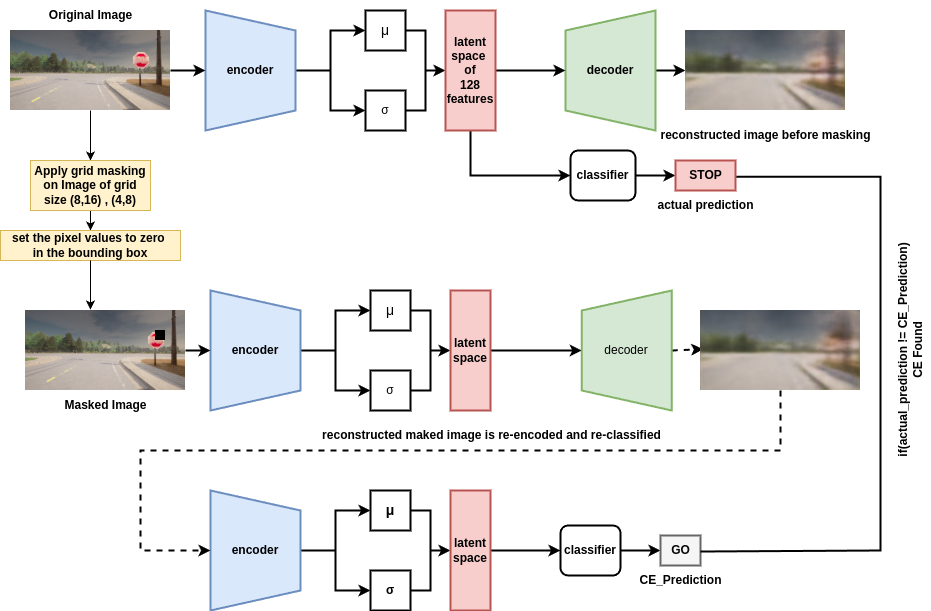
\includegraphics[width=0.95\textwidth]{img/masking/grid_based_masking/grid_based_masking_flow.drawio.png}
\caption{
Workflow of the grid-based counterfactual generation process. Grid cells are masked sequentially in two stages: a fine grid ($8 \times 16$) and a coarse grid ($4 \times 8$). Masked images are reconstructed using a VAE and re-evaluated by the classifier. A prediction change implies that the masked region was causally important.
}
\label{fig:grid_masking_diagram}
\end{figure}

The masking follows a sequential strategy, beginning with the finer grid. Each cell is masked individually by zeroing its pixel values. If masking any one cell results in a change in the model’s prediction, a counterfactual is deemed to have been found, and the process terminates early. This behavior adheres to the principle of \textit{minimal intervention}~\cite{wachter2018CE}, wherein the smallest possible change is sufficient to alter the decision. If no counterfactual is detected in the fine grid, the search continues with the coarse grid.

Once a cell is masked, the resulting image is passed through the encoder-decoder pipeline to maintain visual plausibility. The reconstructed image is then re-encoded and classified. A prediction change signifies that the masked region played a decisive role in the original decision, and thus constitutes a valid counterfactual explanation.


\vspace{1em}
\begin{algorithm}[htbp]
\caption{Grid-Based Masking for Counterfactual Generation}
\label{alg:grid_based_masking}
\begin{algorithmic}[1]
\REQUIRE Image $I$, encoder $E$, decoder $D$, classifier $C$, grid configurations $G = \{(8,16), (4,8)\}$
\ENSURE Whether a counterfactual explanation is found

\STATE Encode image: $z \leftarrow E(I)$
\STATE Predict original label: $y_{\text{orig}} \leftarrow \arg\max C(z)$

\FOR{each grid size $(m, n)$ in $G$}
    \STATE $T \leftarrow m \times n$
    \FOR{$p = 0$ to $T - 1$}
        \STATE Mask grid cell $p$ in $I$ to obtain $I_{\text{masked}}$
        \STATE Encode: $z_{\text{masked}} \leftarrow E(I_{\text{masked}})$
        \STATE Decode: $I_{\text{recon}} \leftarrow D(z_{\text{masked}})$
        \STATE Re-encode: $z_{\text{re}} \leftarrow E(I_{\text{recon}})$
        \STATE Predict: $y_{\text{new}} \leftarrow \arg\max C(z_{\text{re}})$
        \IF{$y_{\text{new}} \neq y_{\text{orig}}$}
            \RETURN Counterfactual explanation found
        \ENDIF
    \ENDFOR
\ENDFOR

\RETURN No counterfactual explanation found
\end{algorithmic}
\end{algorithm}
\vspace{1em}




Figure~\ref{fig:grid_masking_diagram} illustrates the complete grid-based masking workflow. It highlights how the original image is masked, reconstructed, and re-classified. A prediction change from \texttt{STOP} to \texttt{GO} following the masking of a grid cell demonstrates the effectiveness of this approach in revealing causally salient regions. The masked region is processed through a VAE to maintain visual plausibility, ensuring that the model’s reaction is not triggered by implausible image artifacts.

\begin{figure}[htbp]
\centering
\begin{subfigure}[b]{0.3\textwidth}
    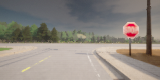
\includegraphics[width=\textwidth]{img/masking/grid_based_masking/original.png}
    \caption{Original Image}
    \label{fig:grid_orig}
\end{subfigure}
\hfill
\begin{subfigure}[b]{0.3\textwidth}
    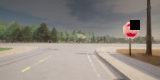
\includegraphics[width=\textwidth]{img/masking/grid_based_masking/reconstructed_grid_masked_image.png}
    \caption{Masked Grid Region}
    \label{fig:grid_masked}
\end{subfigure}
\hfill
\begin{subfigure}[b]{0.3\textwidth}
    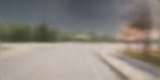
\includegraphics[width=\textwidth]{img/masking/grid_based_masking/CE_grid.png}
    \caption{Reconstructed CE Image}
    \label{fig:grid_recon}
\end{subfigure}
\caption{
Counterfactual explanation generated using grid-based masking. (a) The original image is classified as \texttt{STOP}. (b) A specific grid cell overlapping the STOP sign is masked (blackout). (c) The masked image is reconstructed using a VAE, and reclassified as \texttt{GO}. The change in prediction indicates that the masked region contained causally important features responsible for the initial decision. This result exemplifies the effectiveness of spatial masking in isolating minimal influential regions.
}
\label{fig:grid_ce_example}
\end{figure}

Figure~\ref{fig:grid_ce_example} illustrates the counterfactual generation process using the proposed grid-based masking method. A fine grid is applied to the original image, and each cell is evaluated sequentially. In this instance, masking a specific cell overlapping the STOP sign caused the classifier to change its prediction from \texttt{STOP} to \texttt{GO}. This confirms that the masked region was essential to the model’s decision. The reconstructed image, generated via a Variational Autoencoder, remains visually plausible, ensuring that the change in classification is not due to unrealistic input artifacts.




\subsection{Object Detection-Based Masking} \label{sec:object_detection_masking}

Object Detection-Based Masking introduces a semantically informed approach for generating counterfactual explanations by selectively removing identifiable real-world objects from complex driving scenes. The motivation behind this method is grounded in the causal interpretability of autonomous systems: understanding which specific entities—such as traffic signs, vehicles, pedestrians, or road infrastructure—directly influence a model's driving decision can provide actionable insights into the model's internal reasoning.

Following the general masking pipeline described in Section~\ref{sec:feature_masking_pipeline}, this approach utilizes a Variational Autoencoder (VAE) to encode the original input image into a latent space, which is then passed through a classifier to obtain the model’s initial prediction. However, rather than relying on low-level spatial patterns (as in grid-based masking), this method employs semantic object detection to guide the masking process.

To achieve this, a pre-trained YOLOv5 model~\cite{jocher2020yolov5} is integrated into the pipeline to detect and localize objects present in the input image. The full workflow is illustrated in Figure~\ref{fig:object_detection_workflow}, combining object detection, VAE-based reconstruction, and classifier re-evaluation to identify counterfactuals. YOLOv5 is a single-stage object detector known for its speed and accuracy across 80 COCO classes~\cite{lin2015microsoftcococommonobjects}, including vehicles, persons, and traffic control elements. Each detected object is described by a bounding box $(x_{\min}, y_{\min}, x_{\max}, y_{\max})$, which defines the region to be masked. The overall procedure is summarized in Algorithm~\ref{alg:object_detection_masking}.

\begin{figure}
    \centering
    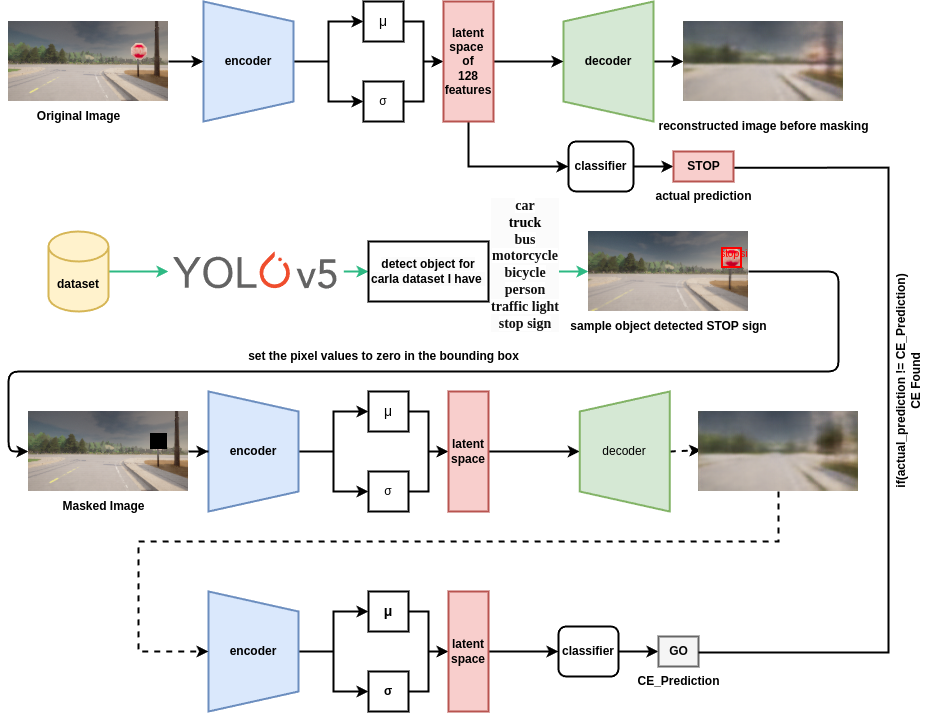
\includegraphics[width=0.95\textwidth]{img//masking//object_detection/object_detection_based_masking_flow.drawio.png}
    \caption{
Workflow of the object detection-based counterfactual explanation pipeline. The input image is first encoded using a Variational Autoencoder (VAE) to obtain a latent representation. The classifier predicts the original driving decision (e.g., \texttt{STOP}). Simultaneously, a pre-trained YOLOv5 detector identifies objects in the image. One detected object (e.g., a STOP sign) is masked and passed through the encoder-decoder pipeline to reconstruct a visually plausible image. If reclassification of this reconstruction results in a different label (e.g., \texttt{GO}), a counterfactual explanation is found. The process is iterated per object, and the first valid counterfactual is retained.
}
\label{fig:object_detection_workflow}
\end{figure}

For each image, the process proceeds iteratively over all detected objects. The pixels inside the bounding box are zeroed out—effectively removing the object from the scene. This masked image is then processed through the VAE's encoder-decoder pipeline and re-classified. If the model's output label changes compared to the original prediction, a counterfactual explanation is said to have been generated. To adhere to the principle of minimal intervention~\cite{wachter2018CE}, only the first successful object level perturbation that triggers a label change is retained per image, ensuring a sparse and interpretable explanation.

In cases where multiple objects are detected but none cause the decision to flip, the method concludes that no object-level counterfactual exists for that specific scene. Additionally, if no objects are detected, the image is skipped from object-based masking consideration.

\vspace{1em}
\begin{algorithm}[H]
\caption{Object Detection-Based Masking for Counterfactual Generation}
\label{alg:object_detection_masking}
\begin{algorithmic}[1]
\REQUIRE Input image $I$, encoder $E$, decoder $D$, classifier $C$, object detector $Y$
\ENSURE Decision on whether a counterfactual explanation is found

\STATE Encode image: $z \leftarrow E(I)$
\STATE Predict original label: $y_{\text{orig}} \leftarrow \arg\max C(z)$
\STATE Detect objects using YOLO: $\mathcal{B} \leftarrow Y(I)$
\IF{$\mathcal{B}$ is empty}
    \RETURN No objects detected; no masking applied
\ENDIF
\FOR{bounding box $(x_{\min}, y_{\min}, x_{\max}, y_{\max}) \in \mathcal{B}$}
    \STATE Mask region in $I$ to obtain $I_{\text{masked}}$
    \STATE Encode: $z_{\text{masked}} \leftarrow E(I_{\text{masked}})$
    \STATE Decode: $I_{\text{recon}} \leftarrow D(z_{\text{masked}})$
    \STATE Re-encode: $z_{\text{re}} \leftarrow E(I_{\text{recon}})$
    \STATE Predict: $y_{\text{new}} \leftarrow \arg\max C(z_{\text{re}})$
    \IF{$y_{\text{new}} \neq y_{\text{orig}}$}
        \RETURN Counterfactual explanation found
    \ENDIF
\ENDFOR
\RETURN No counterfactual explanation found
\end{algorithmic}
\end{algorithm}
\vspace{1em}

This method brings semantic granularity to counterfactual explanation by connecting decisions with real-world entities, offering both interpretability and traceability. This is particularly valuable in autonomous driving, where decisions must often be justified not only in terms of performance but also in terms of safety-critical rationale.

\begin{figure}[htbp]
\centering
\begin{subfigure}[b]{0.24\textwidth}
    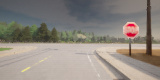
\includegraphics[width=\textwidth]{img/masking/object_detection/original.png}
    \caption{Original Image}
    \label{fig:orig}
\end{subfigure}
\hfill
\begin{subfigure}[b]{0.24\textwidth}
    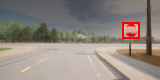
\includegraphics[width=\textwidth]{img/masking/object_detection/with_bbox.png}
    \caption{Object detected}
    \label{fig:orig_bbox}
\end{subfigure}
\hfill
\begin{subfigure}[b]{0.24\textwidth}
    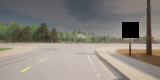
\includegraphics[width=\textwidth]{img/masking/object_detection/masked.png}
    \caption{Masked Image}
    \label{fig:masked}
\end{subfigure}
\hfill
\begin{subfigure}[b]{0.24\textwidth}
    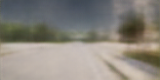
\includegraphics[width=\textwidth]{img/masking/object_detection/CE.png}
    \caption{Reconstructed Image}
    \label{fig:reconstructed}
\end{subfigure}
\caption{
Counterfactual generation through object detection-based masking in a CARLA driving scene. (a) The original image as captured. (b) A STOP sign is detected and localized using YOLOv5. (c) The STOP sign is masked by zeroing out its bounding box. (d) The masked image is reconstructed using a Variational Autoencoder (VAE). The classifier changes its prediction from \texttt{STOP} to \texttt{GO}, indicating that the STOP sign was a causally decisive feature in the original decision.
}
\label{fig:object_detection_masking}
\end{figure}


Figure~\ref{fig:object_detection_masking} illustrates a concrete example of the object detection based masking process applied to a realistic driving scenario. The scene was rendered in the CARLA simulator and contains a STOP sign located on the right-hand side of the road.

The unaltered version of the image (Figure~\ref{fig:orig}) corresponds to the model's original input, for which the classifier predicts the label \texttt{STOP} with high confidence. The YOLOv5 object detector accurately identifies and localizes the STOP sign (Figure~\ref{fig:orig_bbox}), represented by a red bounding box. This is a safety-critical decision, expected in the presence of a regulatory traffic sign.

To probe the causal influence of the STOP sign, the region corresponding to the bounding box is zeroed out (Figure~\ref{fig:masked}). This masked image is then passed through a Variational Autoencoder (VAE), which reconstructs the image in a smooth and naturalistic manner (Figure~\ref{fig:reconstructed}). The reconstruction effectively blurs or removes the masked STOP sign, preserving the surrounding context to remain within the data manifold.

Upon re-encoding and classifying the reconstructed image, the model changes its decision from \texttt{STOP} to \texttt{GO}. This prediction flip signifies a valid counterfactual explanation: the STOP sign was a critical feature in the model’s decision process. Its removal induced a behavioral shift, indicating a direct causal pathway between the visual presence of the STOP sign and the predicted driving action.

This example validates the semantic sensitivity of the proposed method. It reveals that object detection-based masking can expose model dependencies on interpretable, high-level visual cues, facilitating transparency in AI-driven navigation systems.





\subsection{LIME on Images} \label{sec:lime_on_images}

Local Interpretable Model-Agnostic Explanations (LIME) is an explainability framework that identifies which parts of an input image are most responsible for a model’s prediction~\cite{Ribeiro2018}. It achieves this by creating local perturbations typically through masking superpixels and observing how the model’s outputs respond. In this method, we integrate LIME directly into the counterfactual generation pipeline by masking the most influential visual regions and checking whether this perturbation leads to a change in the classifier’s decision.

The primary goal is to determine whether removing highly influential visual features, as identified by LIME, can lead to a change in prediction. If the prediction changes, this minimal perturbation is interpreted as a counterfactual explanation (CE), highlighting that the masked region played a causal role in the original decision.

The method follows the unified image masking pipeline introduced in Section~\ref{sec:feature_masking_pipeline}. First, the input image is passed through a Variational Autoencoder (VAE) to obtain a latent representation, which is classified using a downstream classifier. LIME is then applied to the raw input image to compute a saliency mask that highlights the top-$k$ positively contributing superpixels (we use $k=5$). These superpixels represent regions most influential to the classifier’s predicted label.

Rather than masking regions using hard blackouts or noise, we adopt a soft alpha-blending strategy to ensure that the perturbed image remains realistic and within the data manifold. Formally, the masked image is computed as:
\[
I_{\text{masked}} = (1 - \alpha) \cdot I + \alpha \cdot B \cdot M,
\]
where $I$ is the input image, $M$ is the binary mask from LIME, $B$ is a black background, and $\alpha$ is the blending factor (set to 0.5 in our experiments). This approach mitigates sharp edges or unnatural patterns in the masked image and improves the quality of subsequent reconstructions.

The softly masked image is then passed through the VAE encoder to obtain a latent vector, which is decoded to reconstruct a realistic image. The reconstructed image is re-encoded and passed again to the classifier. If the predicted label changes after this reconstruction process, the masked region is considered causally decisive, and the outcome is recorded as a counterfactual explanation.

Although LIME operates on image space, it does not explain the VAE instead, instead, it explains the classifier that operates on the VAE’s latent space. The predictive function passed to LIME consists of two components. First, the perturbed image is encoded by the VAE encoder to obtain a latent vector. Second, this vector is fed into the classifier to compute prediction probabilities. LIME then perturbs the input image and learns a local linear surrogate model to identify which superpixels influence the output the most. The decoder is used only after masking to produce a visually plausible image for counterfactual evaluation (see Figure~\ref{fig:lime_image_workflow}).

\begin{figure}
    \centering
    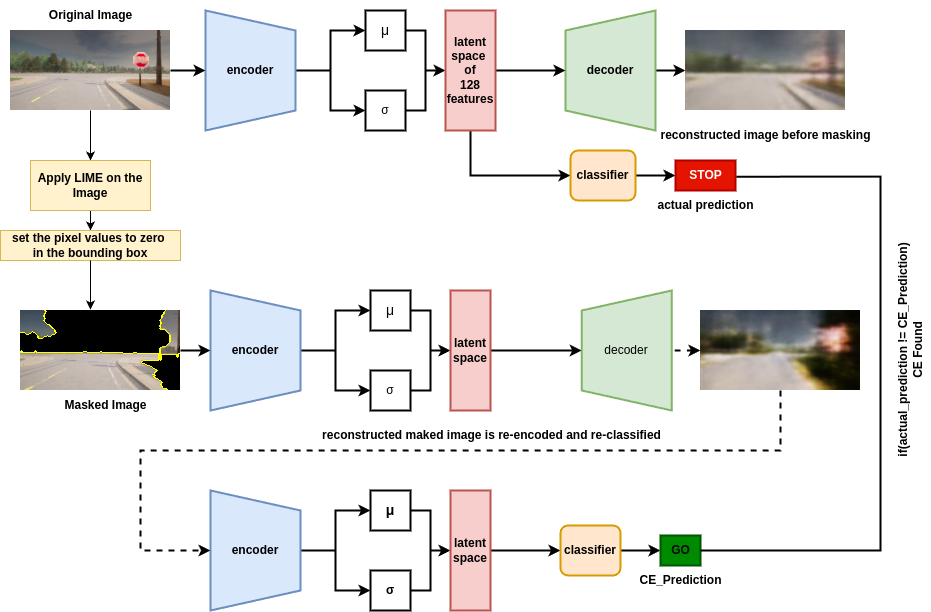
\includegraphics[width=0.95\textwidth]{img/masking/lime_on_images/lime_on_images_based_masking_flow.drawio.png}
    \caption{
Workflow of the LIME-based counterfactual explanation pipeline. The input image is first encoded using a Variational Autoencoder (VAE) to obtain a latent representation, which is classified to produce the original label (e.g., \texttt{STOP}). LIME is then applied to the image to identify the most influential superpixels. These regions are softly masked via alpha blending and passed through the encoder-decoder pipeline for reconstruction. The reconstructed image is re-encoded and re-classified. If the classifier’s prediction changes (e.g., from \texttt{STOP} to \texttt{GO}), a counterfactual explanation is found.
}
\label{fig:lime_image_workflow}
\end{figure}

Our design is motivated by the work of Agarwal and Nguyen~\cite{agarwal2020explainingimageclassifiersremoving}, who proposed combining attribution methods such as LIME with generative inpainting to maintain visual coherence in masked images. While they focus on improving attribution maps using DeepFill-style pretrained inpainters, we propose a complementary pipeline using a domain-specific VAE trained on our driving dataset. Unlike their attribution centric approach, our goal is to explicitly generate counterfactuals minimal and plausible changes that cause a prediction shift. Moreover, our pipeline integrates the VAE not only for reconstruction but also for re-encoding, enabling end-to-end analysis within a single generative framework.

\vspace{1em}
\begin{algorithm}[H]
\caption{LIME on Images for Counterfactual Generation}
\label{alg:lime_on_images}
\begin{algorithmic}[1]
\REQUIRE Image $I$, encoder $E$, decoder $D$, classifier $C$, LIME explainer $L$
\ENSURE Whether a counterfactual explanation is found

\STATE Encode image: $z \leftarrow E(I)$
\STATE Predict original label: $y_{\text{orig}} \leftarrow \arg\max C(z)$

\STATE Generate LIME explanation: $M \leftarrow L(I, C)$
\STATE Select top-$k$ regions: $R \leftarrow \text{Mask}(M, k=5)$
\STATE Apply alpha-blended masking: $I_{\text{masked}} \leftarrow \text{Blend}(I, R, \alpha=0.5)$

\STATE Encode: $z_{\text{masked}} \leftarrow E(I_{\text{masked}})$
\STATE Decode: $I_{\text{recon}} \leftarrow D(z_{\text{masked}})$
\STATE Re-encode: $z_{\text{re}} \leftarrow E(I_{\text{recon}})$
\STATE Predict new label: $y_{\text{new}} \leftarrow \arg\max C(z_{\text{re}})$

\IF{$y_{\text{new}} \neq y_{\text{orig}}$}
    \RETURN Counterfactual explanation found
\ENDIF

\RETURN No counterfactual explanation found
\end{algorithmic}
\end{algorithm}
\vspace{1em}

Unlike grid-based or object detection-based masking, LIME offers a data-driven, input adaptive strategy. It focuses only on regions most important for each specific image, improving interpretability and relevance. However, this comes at a higher computational cost due to multiple sampling and repeated model inference. Despite this, the method’s local precision and model-agnostic formulation make it well-suited for analyzing safety-critical systems like autonomous vehicles.





\subsection{LIME-Based Masking on Latent Features} \label{sec:lime_based_masking_on_latent_features}

\subsubsection*{Latent Feature Statistics Preprocessing}
\label{sec:latent_statistics_preprocessing}
Before applying LIME-based masking in the latent space, it is essential to establish dataset level statistical priors for each latent dimension. This ensures that when latent features are perturbed or replaced, the substituted values remain within a plausible range, preserving semantic consistency.

To compute these priors, all images from the training and test sets are encoded using the trained Variational Autoencoder (VAE) encoder, yielding a 128-dimensional latent vector for each image. The collection of these vectors across the dataset is used to compute per-dimension statistics, including the mean, median, minimum, maximum, and standard deviation.

These computed statistics are used during the masking phase to replace influential latent features. For instance, if LIME identifies a latent dimension as critical to the current classification, its value can be substituted with the median or mean value from the dataset to simulate a more neutral configuration. This strategy ensures that the modified latent vectors remain close to the data manifold, improving the realism of generated counterfactuals.

These statistics serve as the foundation for the LIME on Latent Features method and its Nearest Unchanged Neighbor (NUN) extension.


\subsection{LIME on Latent Features}
\label{sec:lime_on_latent}

This method applies the LIME (Local Interpretable Model-Agnostic Explanations) algorithm directly to the latent space of a trained Variational Autoencoder (VAE) to identify and mask the most influential latent dimensions contributing to the model's classification. Unlike image-space LIME, this approach operates on the compressed latent representation $z \in \mathbb{R}^{128}$, thereby enabling counterfactual reasoning at a more abstract and semantically meaningful level.

Prior to this step, dataset-level statistics such as the median of each latent dimension are computed and stored, as described in Section~\ref{sec:latent_statistics_preprocessing}. These median values, denoted as $\bar{z} \in \mathbb{R}^{128}$, are used as neutral replacements for feature masking.

As shown in the workflow in Figure~\ref{fig:lime_latent_workflow}, the VAE encoder maps the input image $I$ into a latent representation $z = E(I)$. A downstream neural classifier $C$ then provides the prediction $\hat{y}_{\text{orig}} = \arg\max C(z)$. LIME is applied on this latent vector to compute a local linear approximation of the classifier’s decision boundary and returns a list of tuples $\{(w_i, i)\}$, where $w_i$ is the importance weight of the $i$-th latent feature.

Only the positively influential features (i.e., $w_i > 0$) are considered for masking. This choice ensures that we are suppressing features that actively contribute toward the current classification. Replacing negatively influential features (those working against the current class) would potentially reinforce the current decision and thus contradict the goal of counterfactual generation.

The positively weighted features are sorted in descending order of importance, i.e., from the most impactful dimension to the least. Let $\mathcal{F} = \{i_1, i_2, \dots, i_k\}$ denote the ordered set of positively contributing latent feature indices. For each $i \in \mathcal{F}$, the feature $z_i$ is replaced by the corresponding dataset-level median $\bar{z}_i$:

\[
z_i^{\text{masked}} = 
\begin{cases}
\bar{z}_i & \text{if } i \in \mathcal{F}_{\text{used}} \\
z_i & \text{otherwise}
\end{cases}
\]

The modified latent vector is then passed through the decoder to reconstruct an image $I_{\text{recon}} = D(z^{\text{masked}})$. This image is re-encoded and classified again to obtain a new prediction $\hat{y}_{\text{new}} = \arg\max C(E(I_{\text{recon}}))$. If $\hat{y}_{\text{new}} \ne \hat{y}_{\text{orig}}$, the explanation is accepted as a valid counterfactual.

\begin{figure}
    \centering
    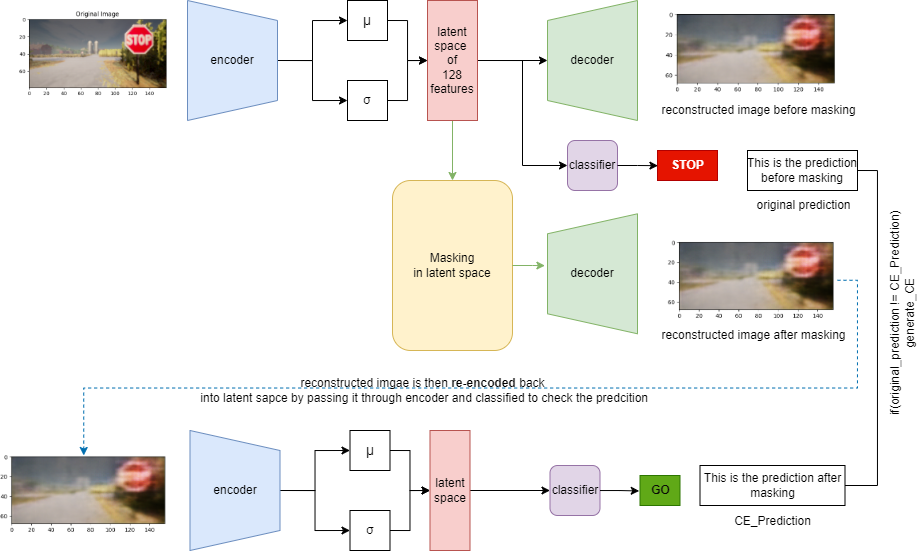
\includegraphics[width=0.95\linewidth]{img//masking//lime_on_latent/LIME_on_latent_space_masking.drawio.png}
    \caption{Enter Caption}
    \label{fig:lime_latent_workflow}
\end{figure}

The full procedure is detailed in Algorithm~\ref{alg:lime_on_latent}, and the complete masking pipeline is illustrated in Figure~\ref{fig:lime_latent_workflow}. This approach ensures semantic plausibility by leveraging dataset-informed statistics and offers a high-level explanation by manipulating deep features learned through the VAE.


\vspace{1em}
\begin{algorithm}[H]
\caption{LIME-Based Masking on Latent Features}
\label{alg:lime_on_latent}
\begin{algorithmic}[1]
\REQUIRE Image $I$, encoder $E$, decoder $D$, classifier $C$, median latent vector $\bar{z}$
\ENSURE Whether a counterfactual explanation is found

\STATE $z \leftarrow E(I)$ \hfill // Encode image to latent vector
\STATE $y_{\text{orig}} \leftarrow \arg\max C(z)$ \hfill // Original prediction

\STATE Use LIME to compute feature importance scores on $z$
\STATE Select positively influential features $\mathcal{F}$, sorted by importance
\FOR{feature index $i$ in $\mathcal{F}$}
    \STATE $z_{\text{masked}} \leftarrow z$ with $z_i \leftarrow \bar{z}_i$
    \STATE $I_{\text{recon}} \leftarrow D(z_{\text{masked}})$
    \STATE $z_{\text{re}} \leftarrow E(I_{\text{recon}})$
    \STATE $y_{\text{new}} \leftarrow \arg\max C(z_{\text{re}})$
    \IF{$y_{\text{new}} \neq y_{\text{orig}}$}
        \RETURN Counterfactual explanation found
    \ENDIF
\ENDFOR

\RETURN No counterfactual explanation found
\end{algorithmic}
\end{algorithm}
\vspace{1em}

This method provides a more abstract yet powerful mechanism for generating counterfactuals, as it operates on high-level learned features. The use of dataset-informed median values ensures semantic consistency, while early stopping improves efficiency. Interpretability is further enhanced by generating visualizations such as LIME importance bar plots and masked feature maps, which are discussed in the Evaluation and Results section.






\subsection{LIME-Based Masking on Latent Features using NUN} \label{lime_with_NUN}


In this work, we extend the counterfactual explanation strategy introduced by Wijekoon et al.~\cite{WijekoonWNMPC21} to the domain of deep generative models. While originally applied to tabular data, we adapt their approach to the latent space of image representations learned by a Variational Autoencoder (VAE). Specifically, we implement \textbf{Method 2}, in which LIME is applied to the latent vector of a \textit{Nearest Unlike Neighbor} (NUN) to guide feature replacement in the query representation until a class change is achieved.


Given an input image \( x \), we encode it into a latent vector \( z \) using a pretrained VAE encoder \( E \), and obtain its predicted class \( y = \arg\max C(z) \) from a trained classifier \( C \). We then identify the Nearest Unlike Neighbor \( \hat{z} \), which belongs to a different predicted class \( \hat{y} \ne y \), by computing the Euclidean distance in the latent space:

\[
\hat{z} = \arg\min_{z_j \in \mathcal{D}_{\text{test}}} \left\{ \| z - z_j \|_2 \; \middle| \; C(z_j) \ne y \right\}
\]

This NUN latent vector represents a semantically close alternative that results in a different classification outcome, and thus serves as a candidate for counterfactual generation.


To prioritize the most relevant feature changes, we apply the \textit{LIME Tabular Explainer}~\cite{Ribeiro2018} on the NUN vector \( \hat{z} \). LIME generates a local surrogate model that assigns importance weights to each latent feature, resulting in an ordered list:

\[
\text{AFOrderLIME}(\hat{z}) = \{ i_1, i_2, \dots, i_m \}, \quad \text{where } |w_{i_1}| > |w_{i_2}| > \dots > |w_{i_m}|
\]

These weights indicate how much each latent feature contributes to the predicted class of the NUN. We use this ranking to iteratively transfer features from \( \hat{z} \) to \( z \).


Following the LIME importance order, we replace each latent dimension \( z[i_k] \leftarrow \hat{z}[i_k] \) and reconstruct the modified latent vector \( z' \). The reconstruction \( x' = D(z') \) is passed through the encoder and classifier again to determine whether a class change has occurred. This process continues until the prediction flips, ensuring that we identify a minimal set of feature modifications necessary to generate a counterfactual. The complete procedure is presented in Algorithm~\ref{alg:nun_lime}

\begin{figure}[htbp]
    \centering
    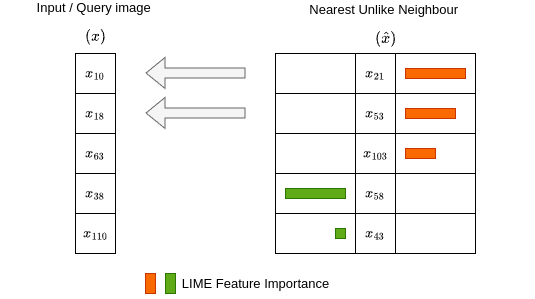
\includegraphics[width=0.55\textwidth]{img/masking/lime_on_latent_nun/NUN_method.drawio.png}
    \caption{Illustration of the proposed method. Important latent features (as determined by LIME) are transferred from the NUN to the input in order of decreasing importance until the classifier's prediction changes.}
    \label{fig:nun_lime}
\end{figure}


An illustration of this feature transfer mechanism is shown in Figure~\ref{fig:nun_lime}. The left column depicts the latent features of the input image, while the right column represents the features of its NUN. LIME-assigned importance is indicated through color-coded bars. Features with higher importance are prioritized during transfer from the NUN to the input. Arrows between the two vectors highlight the flow of values during the masking process.




\begin{algorithm}[htbp]
\caption{LIME-Based Masking on Latent Features using NUN}
\label{alg:nun_lime}
\begin{algorithmic}[1]
\REQUIRE Encoder $E$, Decoder $D$, Classifier $C$, Query image $I$, Test dataset $\mathcal{D}_{\text{test}}$, Label mapping $\mathcal{L}$
\ENSURE Counterfactual image $x_{\text{cf}}$, Number of features replaced $k$, Evaluation metrics

\STATE $z \leftarrow E(I)$ \hfill \textit{// Encode query to latent space}
\STATE $y \leftarrow \arg\max C(z)$ \hfill \textit{// Get predicted label}
\STATE $z_{\text{NUN}} \leftarrow \text{None}$, $d_{\min} \leftarrow \infty$

\FORALL{$J \in \mathcal{D}_{\text{test}}$}
    \STATE $z_j \leftarrow E(J)$
    \STATE $y_j \leftarrow \arg\max C(z_j)$
    \IF{$y_j \ne y$}
        \STATE $d \leftarrow \|z - z_j\|_2$
        \IF{$d < d_{\min}$}
            \STATE $z_{\text{NUN}} \leftarrow z_j$
            \STATE $d_{\min} \leftarrow d$
        \ENDIF
    \ENDIF
\ENDFOR

\STATE $\text{importance} \leftarrow \text{LIME}(z_{\text{NUN}}, C)$
\STATE $\mathcal{F} \leftarrow \text{SortDescendingByImportance}(\text{importance})$
\STATE $z_{\text{mod}} \leftarrow z$, $k \leftarrow 0$

\FORALL{$i \in \mathcal{F}$}
    \STATE $z_{\text{mod}}[i] \leftarrow z_{\text{NUN}}[i]$
    \STATE $x_{\text{recon}} \leftarrow D(z_{\text{mod}})$
    \STATE $z_{\text{reenc}} \leftarrow E(x_{\text{recon}})$
    \STATE $y_{\text{new}} \leftarrow \arg\max C(z_{\text{reenc}})$
    \STATE $k \leftarrow k + 1$
    \IF{$y_{\text{new}} \ne y$}
        \STATE \textbf{break}
    \ENDIF
\ENDFOR

\STATE $\text{metrics} \leftarrow \text{Evaluate}(I, x_{\text{recon}})$
\RETURN $x_{\text{recon}}, k, \text{metrics}$
\end{algorithmic}
\end{algorithm}


This approach leverages LIME’s interpretability and the semantic richness of the latent space to generate actionable counterfactuals. It ensures minimal intervention while maintaining high visual fidelity, and directly aligns with the counterfactual generation principles outlined by Wijekoon et al.~\cite{WijekoonWNMPC21}.







